\chapter{Psalm 28}

\begin{figure}
  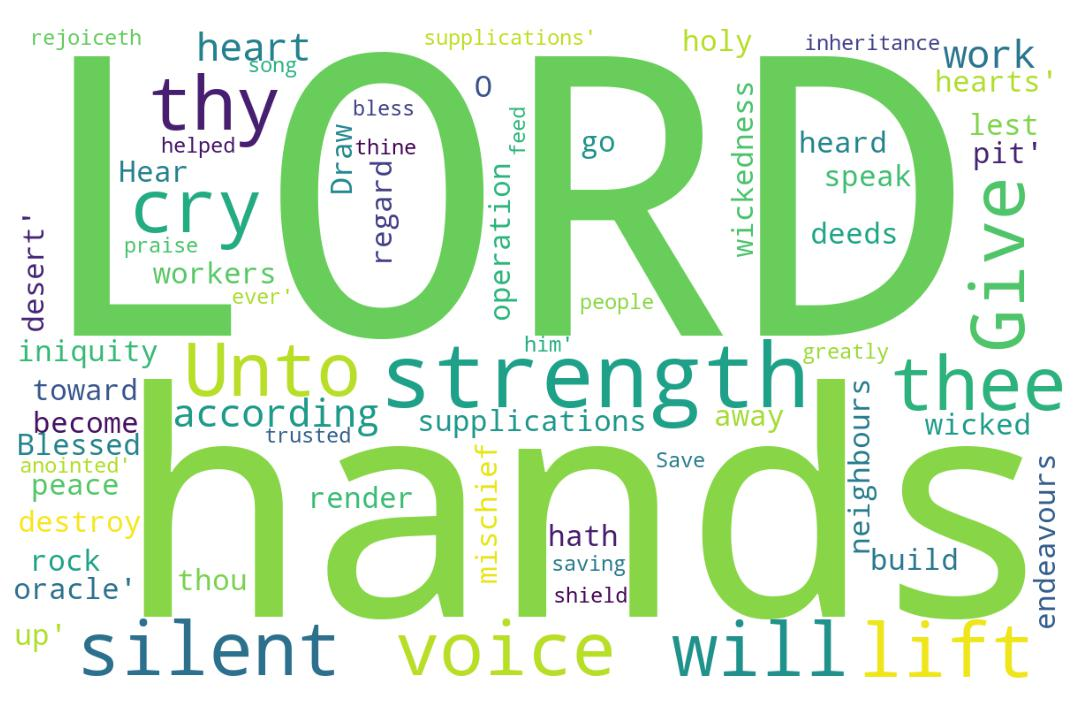
\includegraphics[width=\linewidth]{19OT-Psalms/Psalm28-WordCloud.jpg}
  \caption{Psalm 28 Word Cloud}
  \label{fig:Psalm 28 word Cloud}
\end{figure}

\marginpar{\scriptsize \centering \fcolorbox{bone}{lime}{\textbf{A VERY PERSONL FAITH}}\\ (Psalm  28:1--14) \begin{compactenum}[I.][8]
    \item His \textbf{Supplications} \index[scripture]{Psalms!Psa 028:02}\index[scripture]{Psalms!Psa 028:06}(Psa 28:2, 6)
    \item His \textbf{Surety} \index[scripture]{Psalms!Psa 028:05}(Psa 28:5)
    \item His \textbf{Song} \index[scripture]{Psalms!Psa 028:07}(Psa 28:7)
    \item His \textbf{Strength} \index[scripture]{Psalms!Psa 028:07}\index[scripture]{Psalms!Psa 028:08}(Psa 28:7, 8)
    \item His \textbf{Shield} \index[scripture]{Psalms!Psa 028:07}(Psa 28:7)
    \item His \textbf{Source} of Rejoicing \index[scripture]{Psalms!Psa 028:07}(Psa 28:7)
    \item His \textbf{Salvation} \index[scripture]{Psalms!Psa 028:08}\index[scripture]{Psalms!Psa 028:09}(Psa 28:8, 9)
\end{compactenum}}

\footnote{\textcolor[cmyk]{0.99998,1,0,0}{\hyperlink{TOC}{Return to end of Table of Contents.}}}\footnote{\href{https://www.audioverse.org/english/audiobibles/books/ENGKJV/O/Ps/1}{\textcolor[cmyk]{0.99998,1,0,0}{Psalms Audio}}}\textcolor[cmyk]{0.99998,1,0,0}{\emph{A Psalm} of David.}\\
\\
\textcolor[cmyk]{0.99998,1,0,0}{Unto thee will I cry, O LORD my rock; be not silent to me: lest, \emph{if} thou be silent to me, I become like them that go down into the pit.}\footnote{Study all the verses that contain the words \textbf{go}, \textbf{down}, and \textbf{pit}. The pit is literally the \textbf{bottomless pit} named in (1) Revelation 9:1, (2) Revelation 9:2, (3) Revelation 9:11, (4) Revelation 11:7, (5) Revelation 17:8, (6) Revelation 20:1, and (7) Revelation 20:3. It  is typified by the pit used to trap Joseph in Genesis 37.}
[2] \textcolor[cmyk]{0.99998,1,0,0}{Hear the voice of my \fcolorbox{bone}{lime}{supplications}, when I cry unto thee, when I lift up my hands toward thy holy oracle.}
[3] \textcolor[cmyk]{0.99998,1,0,0}{Draw me not away with the wicked, and with the workers of iniquity, which speak peace to their neighbours, but mischief \emph{is} in their hearts.}
[4] \textcolor[cmyk]{0.99998,1,0,0}{Give them according to their deeds, and according to the wickedness of their endeavours: give them after the work of their hands; render to them their desert.}
[5] \textcolor[cmyk]{0.99998,1,0,0}{Because they regard not the works of the LORD, nor the operation of his hands, \fcolorbox{bone}{lime}{he shall} destroy them, and not build them up.}
[6] \textcolor[cmyk]{0.99998,1,0,0}{Blessed \emph{be} the LORD, because he hath heard the voice of my supplications.}
[7] \textcolor[cmyk]{0.99998,1,0,0}{The LORD \emph{is} my \fcolorbox{bone}{lime}{strength} and my \fcolorbox{bone}{lime}{shield}; my heart trusted in him, and I am helped: therefore my heart greatly rejoiceth; and with my \fcolorbox{bone}{lime}{song} will I praise him.}
[8] \textcolor[cmyk]{0.99998,1,0,0}{The LORD \emph{is} their \fcolorbox{bone}{lime}{strength}, and he \emph{is} the saving \fcolorbox{bone}{lime}{strength} of his anointed.}
[9] \textcolor[cmyk]{0.99998,1,0,0}{\fcolorbox{bone}{lime}{Save} thy people, and bless thine inheritance: feed them also, and lift them up for ever.}



